\section{System Methodology}
\label{3}
This section presents the PrivSearch framework. We first describe the architectural design principles and the layered system architecture (Section~\ref{3A}), then define the system and adversary model (Section~\ref{3B}), the unified authenticated query framework (Section~\ref{3C}), the replay-protection mechanism (Section~\ref{3D}), the formal security analysis (Section~\ref{3E}), the leakage profile and confidentiality scope (Section~\ref{subsec:leakage}), and the analytical cost model that connects the formal properties to the measured phase timings reported in Section~\ref{4} (Section~\ref{3F}).

\subsection{Design Principles and System Architecture}
\label{3A}
PrivSearch is built around a single architectural invariant: operational query latency must remain decoupled from blockchain anchoring latency. We denote the operational and encrypted search latencies as $T_{search}$ and the asynchronous blockchain anchoring latency as $T_{anchor}$, and require
\begin{equation}
T_{search} \perp T_{anchor},
\label{eq:invariant}
\end{equation}
meaning that read-query latency is architecturally independent of the anchoring queue backlog. This principle is enforced by a five-layer architecture, illustrated in Fig.~\ref{fig:architecture}.

\begin{figure*}[t]
\centering
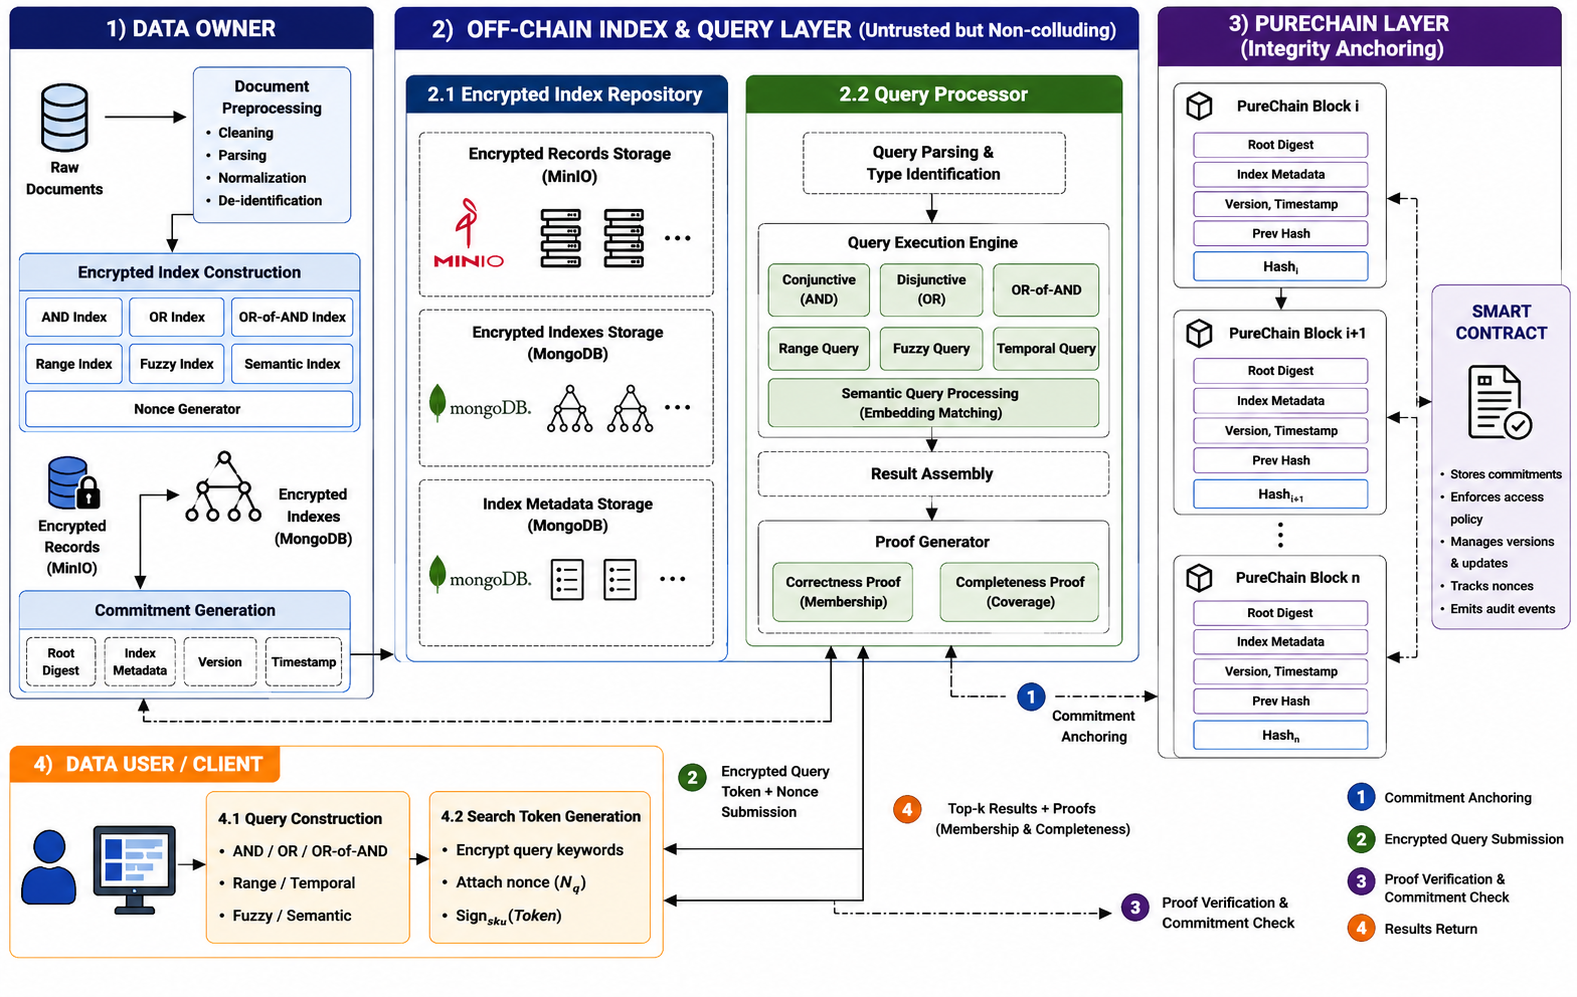
\includegraphics[width=0.92\textwidth]{pics/System Archit.png}
\caption{PrivSearch system architecture. The data owner constructs authenticated conjunctive, disjunctive, OR-of-AND, range, fuzzy, and semantic indexes and anchors commitments on PureChain (left). The off-chain index and query layer executes queries against encrypted storage and generates correctness and completeness proofs (center). PureChain maintains an append-only chain of root digests, index metadata, and a nonce registry for replay detection (right). The data user constructs encrypted queries, submits nonce-bound tokens, and verifies returned proofs before consuming results (bottom).}
\label{fig:architecture}
\end{figure*}

\textbf{Layer 1 (Application layer)} exposes a REST interface for ingestion, query submission, and administrative operations, and is the point at which freshness tuples are attached to every state-mutating request.

\textbf{Layer 2 (Dual-layer index)} is the core architectural contribution. An \emph{operational index} maintains non-sensitive attributes in plaintext B-tree structures for low-latency administrative lookups ($O(\log n + |R|)$), while a \emph{privacy index} maintains an authenticated encrypted index over sensitive keyword and metadata attributes. The privacy index extends the OXT searchable-symmetric-encryption protocol used by SeaCQ~\cite{Yang}, which achieves optimal conjunctive complexity $O(|R_{w_{min}}|)$ by intersecting candidate identifiers around the least-frequent query keyword. Both index paths are designed so that $T_{search} \perp T_{anchor}$ holds independently of anchor-queue state.

\textbf{Layer 3 (Encrypted object storage)} stores AES-256-GCM encrypted record payloads, with a SHA-256 content hash computed prior to encryption and a storage pointer returned to the index layer; plaintext payloads are never persisted in object storage.

\textbf{Layer 4 (Decentralized replication, optional)} allows encrypted replicas to be distributed across content-addressed storage for cross-institution access, with only the content identifier recorded in metadata.

\textbf{Layer 5 (Blockchain integrity layer)} anchors three complementary mechanisms on the PureChain-backed platform: (i) an RSA-accumulator-based authenticated data structure (ADS) that provides per-query correctness and completeness proofs, following the constant-size ADS construction used by SeaCQ$^{*}$ so that on-chain storage is $O(1)$ rather than $O(s_r+s_c)$; (ii) Merkle batch anchoring, in which sealed batches of audit transactions are hashed into a Merkle root and anchored asynchronously, giving $O(1)$ amortized gas cost per batch; and (iii) a nonce registry realized as a sliding-window Bloom filter that performs real-time replay detection at the API boundary, described in Section~III-D. An adaptive anchor scheduler monitors the observed arrival-to-processing ratio $\lambda/\mu$ and adjusts the anchoring batch size $b$ so that backlog growth is bounded without ever blocking the query path, which is the mechanism that operationally realizes Eq.~\eqref{eq:invariant} under bursty write load.

Fig.~\ref{fig:pipeline} shows the corresponding end-to-end query pipeline, from query submission through normalization, trapdoor generation, index search, proof generation, proof verification, and freshness checking, to result delivery. This pipeline is the operational counterpart of the analytical cost model developed in Section~\ref{3F}.

\begin{figure*}[t]
\centering
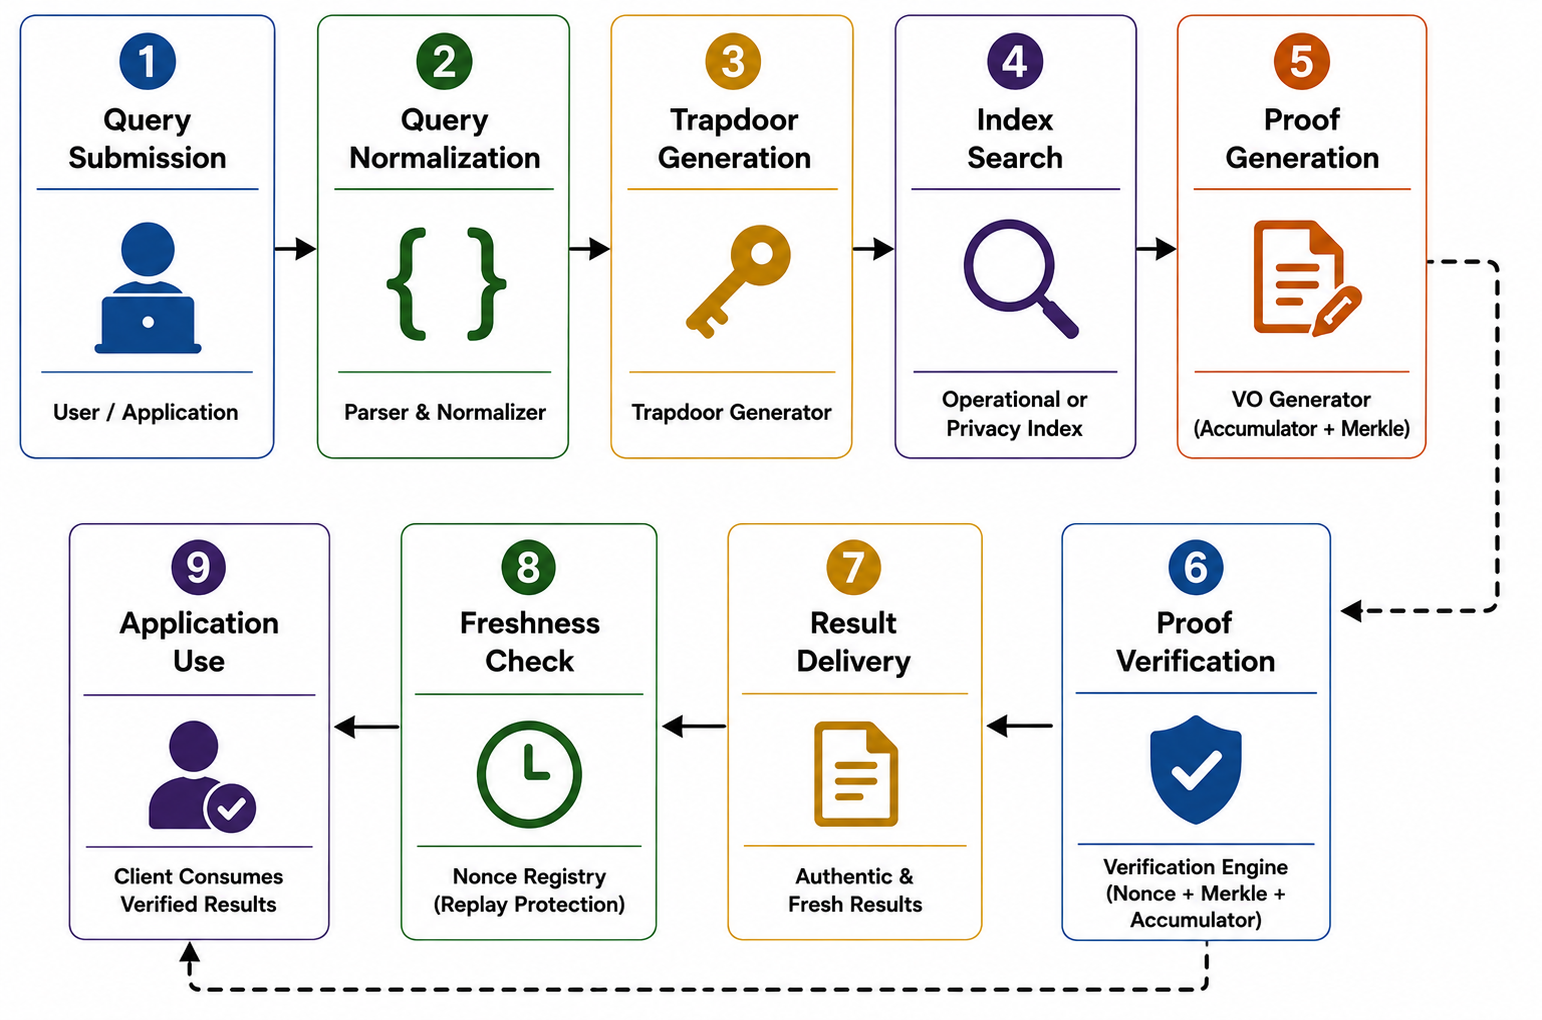
\includegraphics[width=0.92\textwidth]{pics/End to End Query Workflow.png}
\caption{End-to-end PrivSearch query pipeline. Each stage corresponds to one additive term in the analytical latency model of Eq.~\eqref{eq:tquery}: query normalization, trapdoor generation, index search, verification-object (proof) generation, proof verification, and freshness checking against the nonce registry, before authenticated results are returned to the client.}
\label{fig:pipeline}
\end{figure*}

\subsection{System Model and Notation}
\label{3B}
Let $D=\{d_1,\dots,d_n\}$ denote the outsourced document set and $W$ the keyword universe. Let $I(w)$ denote the authenticated posting list for keyword $w \in W$, and let $M(d)$ denote authenticated metadata bound to document $d$ (e.g., month/year buckets used for range queries). Let $\mathrm{Com}(I)$ denote the authenticated commitment of the current index state, anchored on-chain. For a query $Q$, the server returns an answer set $A$ and a proof object $P$; the client-side verifier computes
\begin{equation}
\mathrm{Verify}(Q,A,P,\mathrm{Com}(I)) \in \{\text{accept}, \text{reject}\}.
\end{equation}
We consider four principal query classes: conjunctive $Q_{and}$, disjunctive $Q_{or}$, range $Q_{range}$, and fuzzy $Q_{fuzzy}$, together with a concept-expanded semantic query $Q_{sem}$ described in Section~\ref{3C6}. Every PrivSearch query is expressible in disjunctive normal form (DNF),
\begin{equation}
Q = C_1 \lor C_2 \lor \cdots \lor C_d, \quad
C_i = \bigwedge_{j} (k_j = v_j) \wedge \bigwedge_{l} \big(r_l \in [a_l,b_l]\big),
\label{eq:dnf}
\end{equation}
where each clause $C_i$ is a conjunction of equality predicates over searchable keyword attributes $k_j$ and optional range predicates over attributes $r_l$. The final answer is $A = \bigcup_i \sigma_{C_i}(D)$, deduplicated on document identifier. Table~\ref{tab:acronyms} summarizes the acronyms and abbreviations used throughout the remainder of the paper.
\begin{table}[t]
\centering
\caption{Summary of Acronyms and Abbreviations}
\label{tab:acronyms}
\small
\begin{tabular}{ll}
\toprule
\textbf{Acronym} & \textbf{Full Meaning} \\
\midrule
ADS & Authenticated Data Structure \\
AES & Advanced Encryption Standard \\
API & Application Programming Interface \\
CI & Confidence Interval \\
CPU & Central Processing Unit \\
DNF & Disjunctive Normal Form \\
GCM & Galois/Counter Mode \\
HMAC & Hash-based Message Authentication Code \\
HTTP & Hypertext Transfer Protocol \\
IIoT & Industrial Internet of Things \\
IoMT & Internet of Medical Things \\
$k$NN & $k$-Nearest Neighbor \\
LAN & Local Area Network \\
NDC & National Drug Code \\
P95 / P99 & 95th / 99th Percentile (latency) \\
REST & Representational State Transfer \\
RSA & Rivest--Shamir--Adleman \\
SD & Standard Deviation \\
SHA-256 & Secure Hash Algorithm, 256-bit \\
TEE & Trusted Execution Environment \\
WAN & Wide Area Network \\
\bottomrule
\end{tabular}
\end{table}
We assume the following trust and adversary model, consistent with the semi-honest/malicious cloud model used in prior authenticated blockchain query work~\cite{Yang,Yin,Wu}: the data owner and data user are honest, the blockchain platform is honest and append-only, and the off-chain cloud server (storage and query execution) is potentially malicious it may return incorrect, incomplete, stale, or fabricated results, or attempt to replay previously accepted requests. Table~\ref{tab:threat} summarizes the adversaries considered, their capabilities, and the corresponding PrivSearch mitigation.
\begin{table}[t]
\centering
\caption{Threat Model and Mitigations}
\label{tab:threat}
\scriptsize
\setlength{\tabcolsep}{3pt}
\begin{tabular}{p{1.3cm}p{1.4cm}p{1.55cm}p{1.85cm}}
\toprule
\textbf{Adversary} & \textbf{Goal} & \textbf{Capability} & \textbf{Mitigation} \\
\midrule
Malicious cloud server & Alter, omit, or fabricate results & Controls outsourced storage/query execution & Authenticated postings, proof verification, committed index state \\
Replay attacker & Resubmit accepted writes & Captures/replays valid request material & Nonce-bound freshness checks, replay cache \\
Stale-proof attacker & Return once-valid, outdated proofs & Reuses proof from earlier state & Commitment binding, state-consistency verification \\
Adaptive query adversary & Infer sensitive structure & Chooses queries adaptively from outputs & Leakage bounded by Definition~\ref{def:leakage}; see Theorem~\ref{thm:leakage_security} \\
\bottomrule
\end{tabular}
\end{table}
PrivSearch is evaluated under this outsourced off-chain server model using a runnable prototype integrated with the hybrid blockchain stack, rather than by deploying a physically separate, independently hosted cloud server. Under this model, the completed experiments cover authenticated query execution across all six query families on both the Enron-derived and healthcare corpora, live replay-protection benchmarking against the active API path, resource-overhead measurement of the prototype off-chain engine, and WAN-style distributed-validation benchmarking using real networked validator peers under injected latency and jitter profiles (Section~\ref{4}). A separately hosted, independently deployed public-cloud or remote query-server benchmark, in which the off-chain component runs under a different party's physical infrastructure, is not yet part of the current experimental scope and remains future work.

We do not claim leakage-free secure computation against an adaptive query adversary. Rather, PrivSearch reduces result-tampering, replay, and stale-state risks under an authenticated encrypted-search architecture. As with the OXT family of protocols underlying the privacy index, some access-pattern leakage remains, and this residual leakage is stated explicitly rather than ignored.

\subsection{Authenticated Query Framework}
\label{3C}
PrivSearch supports six query families under the unified DNF model of Eq.~\eqref{eq:dnf}.

\subsubsection{Conjunctive Baseline}
\label{3C1}
The conjunctive query $Q_{and}=w_1 \wedge \cdots \wedge w_k$ follows the OXT-style AND-search model used by SeaCQ: a record is returned only if it belongs to every contributing authenticated posting list $I(w_1),\dots,I(w_k)$. This family is retained as the direct experimental baseline against SeaCQ (Section~\ref{4G}).

\subsubsection{Disjunctive OR Query}
\label{sec:or-query}
PrivSearch processes a disjunctive query by evaluating each constituent
clause independently and combining the authenticated clause-level results:
\begin{equation}
\begin{aligned}
Q_{\mathrm{or}}
    &= c_1 \lor c_2 \lor \cdots \lor c_m,\\
A_{\mathrm{or}}
    &= \bigcup_{i=1}^{m} A(c_i),
    \qquad
A(c_i)=\bigcap_{w\in c_i} I(w).
\end{aligned}
\label{eq:qor}
\end{equation}
Each clause \(c_i\) is evaluated by the conjunctive-query engine and
authenticated against its corresponding posting lists. The final answer
\(A_{\mathrm{or}}\) is obtained by deduplicating the union of all clause
answers that pass verification. Consequently, the client can authenticate
the OR-query result without introducing an additional trusted component.
Algorithm~\ref{alg:authenticated-or} summarizes this procedure.

\begin{algorithm}[t]
\caption{Authenticated OR-Query Evaluation}
\label{alg:authenticated-or}
\begin{algorithmic}[1]
\Require Query $Q_{\mathrm{or}}=c_1\lor\cdots\lor c_m$,
commitment $\mathrm{Com}(I)$
\Ensure Verified answer $A_{\mathrm{or}}$ and proof $P_{\mathrm{or}}$
\State $A_{\mathrm{or}}\gets\emptyset$
\State $P_{\mathrm{or}}\gets\emptyset$
\For{$i=1$ to $m$}
    \State $(A(c_i),P(c_i))
    \gets \Call{EvaluateClause}{c_i}$

    \If{$\mathrm{Verify}\bigl(c_i,A(c_i),P(c_i),
        \mathrm{Com}(I)\bigr)=\mathit{reject}$}
        \State \textbf{abort}
        \Comment{Clause verification failed}
    \EndIf

    \State $A_{\mathrm{or}}\gets
    A_{\mathrm{or}}\cup A(c_i)$
    \Comment{Deduplicate by document ID}

    \State $P_{\mathrm{or}}\gets
    P_{\mathrm{or}}\cup P(c_i)$
\EndFor
\State \Return $(A_{\mathrm{or}},P_{\mathrm{or}})$
\end{algorithmic}
\end{algorithm}

This construction broadens the searchable query language beyond conjunctive-only retrieval while preserving a verifiable result-construction process, rather than simply concatenating unauthenticated clause outputs.

\subsubsection{OR-of-AND Query}
\label{3C3}
PrivSearch further supports small-clause-count disjunctive normal form,
\begin{equation}
Q_{oa} = \bigvee_{i=1}^{p}\Big(\bigwedge_{j=1}^{q_i} w_{ij}\Big), \qquad
A_{oa} = \bigcup_{i=1}^{p}\ \bigcap_{j=1}^{q_i} I(w_{ij}),
\label{eq:qoa}
\end{equation}
e.g., $(w_1 \wedge w_2) \lor (w_3 \wedge w_4)$, which captures realistic ``alternative constrained case'' queries rather than single-keyword alternation alone. Each conjunctive clause is evaluated by the standard AND engine, and the verified clause outputs are combined by the same deduplicated-union procedure as Algorithm~\ref{alg:authenticated-or}.

\subsubsection{Temporal Range Query}
\label{3C4}
Range queries are evaluated over authenticated metadata buckets $M(d)$ keyed by month or year. Let $\mathcal{B}(a,b) = \{\, t : t \text{ is a metadata bucket}, a \le t \le b \,\}$ denote the set of buckets covered by interval $[a,b]$, and let $B(a,b)=|\mathcal{B}(a,b)|$ denote the number of covered buckets. The Rang query engine computes
\begin{equation}
A_{range} = \Big(\bigcup_{t \in \mathcal{B}(a,b)} M^{-1}(t)\Big) \cap \bigcap_{j} I(k_j),
\label{eq:qrange}
\end{equation}
where $M^{-1}(t)=\{d \in D : t \in M(d)\}$ is the set of documents bound to bucket $t$, and the optional intersection with $I(k_j)$ applies any accompanying equality predicates as in Eq.~\eqref{eq:dnf}. PrivSearch (i) resolves $[a,b]$ to the covered bucket set $\mathcal{B}(a,b)$, (ii) retrieves and authenticates postings for each bucket, and (iii) unions and verifies the candidate set. The evaluated workload spans one-, three-, and six-month windows and two-, three-, and five-year windows, so that both selective and broad-coverage temporal behavior is characterized.

\subsubsection{Bounded Fuzzy Matching}
\label{3C5}
Let $ed(w,w')$ denote the edit (Levenshtein) distance between keywords $w,w' \in W$. PrivSearch supports bounded fuzzy keyword matching with edit-distance threshold one,
\begin{equation}
\begin{aligned}
Q_{\mathrm{fuzzy}}(w)
    &= \{\,w' \in W : \operatorname{ed}(w,w') \leq 1\,\},\\
A_{\mathrm{fuzzy}}
    &= \bigcup_{w' \in Q_{\mathrm{fuzzy}}(w)} I(w').
\end{aligned}
\label{eq:qfuzzy}
\end{equation}
so that a query keyword $w$ retrieves the authenticated union of postings for every keyword within one insertion, deletion, or substitution of $w$. This tolerates approximate textual variation while remaining close to authenticated exact-keyword search; it is intentionally a bounded fuzzy model rather than a full similarity search over arbitrary edit distance.

\subsubsection{Semantic Query (v1)}
\label{3C6}
The semantic-search path (\emph{semantic\_v1}) represents a high-level concept $c$ as a curated expansion-term set $E(c)=\{t_1,\dots,t_r\} \subseteq W$ with per-term weights $\omega_1,\dots,\omega_r$. The query engine computes
\begin{equation}
A_{sem} = \bigcup_{t \in E(c)} I(t), \qquad
\mathrm{score}(d) = \!\!\sum_{t \in E(c)\,:\,d \in I(t)}\!\! \omega_t,
\label{eq:qsem}
\end{equation}
expanding the concept into authenticated keyword postings, unioning the candidate set $A_{sem}$, ranking documents by $\mathrm{score}(d)$, and verifying the ranked output against the underlying authenticated postings $I(t)$. This grounds semantic expansion in authenticated keyword postings rather than in a neural embedding index, so that verification remains tractable; it is reported as a first-generation executable semantic path rather than an embedding-based semantic retrieval system.
The expansion set $E(c)$ and its per-term weights $\omega_1,\dots,\omega_r$ reside entirely on the client; only the HMAC-SHA256 keyword trapdoors derived from the elements of $E(c)$ are transmitted to the server, so the concept $c$ itself is never exposed.

\subsection{Replay-Protection Mechanism}
\label{3D}
Every state-mutating request carries a freshness tuple $(nonce, ts, auth)$. A sliding-window Bloom filter the \emph{nonce registry} maintains the set of recently observed nonces over a configurable validity window (e.g., 24 hours for clinical event deduplication):
\begin{equation}
\mathrm{Admit}(n_i)=
\begin{cases}
\text{reject (\texttt{DUPLICATE\_EVENT})} & \\ \text{if } n_i \in \mathrm{BloomFilter} \\
\text{add } n_i;\ \text{process}(event) & \text{otherwise}
\end{cases}
\end{equation}
The check executes \emph{before} any state mutation, so a replayed request cannot cause a second accepted write. The false-positive rate is configurable via filter size and is set below $10^{-3}$\% for the reported experiments. This mechanism directly targets a gap in prior hybrid-blockchain evidence, where replay attempts were previously detectable only after the fact through audit inspection rather than rejected in real time at the request boundary; Section~IV-N reports the corresponding live benchmark.

\subsection{Formal Security Analysis}
\label{3E}
We now state the correctness, completeness, replay-resistance, and latency-separation properties of PrivSearch as definition--theorem--proof triples, connecting each to the corresponding experimental evidence in Section~\ref{4}.

\begin{definition}[Authenticated conjunctive query]
Let $Q_{and}=w_1 \wedge w_2 \wedge \cdots \wedge w_k$. Let $I(w_i)$ denote the committed authenticated posting list for $w_i$, and let $\mathrm{Verify}(Q,A,P)$ accept only if answer set $A$ and proof $P$ are consistent with the committed state $\mathrm{Com}(I)$.
\end{definition}

\begin{theorem}[Conjunctive correctness]
\label{thm:conj_correct}
If $\mathrm{Verify}(Q_{and},A_{and},P_{and})$ accepts, then every document in $A_{and}$ satisfies all conjunctive query terms under the committed dataset state.
\end{theorem}
\begin{proof}
Verifier acceptance implies every posting list used in the answer is authenticated against $\mathrm{Com}(I)$. The query algorithm computes $A_{and}$ only from the intersection $I(w_1)\cap\cdots\cap I(w_k)$. Hence every $d\in A_{and}$ belongs to each authenticated posting list and satisfies all query terms; any document violating a term would fail membership consistency with at least one authenticated posting list, causing rejection.
\end{proof}

\begin{theorem}[Conjunctive completeness]
If $\mathrm{Verify}(Q_{and},A_{and},P_{and})$ accepts, then no valid committed conjunctive result is omitted from $A_{and}$.
\end{theorem}
\begin{proof}
Let $R_{and}=I(w_1)\cap\cdots\cap I(w_k)$ be the true committed answer. Suppose, for contradiction, $d^*\in R_{and}$ but $d^*\notin A_{and}$. Since $d^*$ belongs to every authenticated posting list, its omission is inconsistent with the deterministic intersection induced by the committed state, and the verifier which checks consistency against the authenticated intersection structure rejects. This contradicts acceptance; hence no valid committed result is omitted.
\end{proof}

Theorems 1--2 justify interpreting the zero verification failures observed across all 436 Enron-derived and 258 healthcare-derived non-semantic workloads (Section~\ref{4D}, \ref{4F}) as evidence that the implemented verifier preserves exact authenticated answer recovery under the tested conjunctive workloads.

\begin{definition}[Authenticated OR query]
Let $Q_{or}=c_1\lor c_2\lor\cdots\lor c_m$, where each clause $c_i$ is individually authenticated and the final answer is the deduplicated union of accepted clause answers.
\end{definition}

\begin{theorem}[OR-query correctness]
If each clause answer $A(c_i)$ is accepted by the verifier and the final answer is computed by deduplicated union, the returned OR answer equals the committed OR-query result.
\end{theorem}
\begin{proof}
By clause-level acceptance, $A(c_i)=R(c_i)$ (the true committed clause result) for every $i$. Substituting, $A_{or}=R(c_1)\cup\cdots\cup R(c_m)$. Deduplication removes only repeated identifiers, never unique valid results, and no document failing all clauses can appear in any accepted clause answer. Hence $A_{or}$ equals the true OR-query union.
\end{proof}

\begin{corollary}[Additive OR verification cost]
Authenticated OR execution introduces additive clause-wise proof handling and verification cost across independently verified clauses.
\end{corollary}
This corollary is reflected empirically by the OR-query benchmarks in Section~\ref{4}, which show that authenticated OR support is achieved with sub-millisecond average total latency and zero verification failures across the tested Enron-derived and healthcare workloads.

\begin{definition}[Authenticated temporal range query]
Let $Q_{range}=[a,b]$ be a metadata-backed interval query over authenticated month or year buckets derived from the committed dataset state.
\end{definition}

\begin{theorem}[Range-query correctness]
\label{thm:range_correct}
If $\mathrm{Verify}(Q_{range},A_{range},P_{range})$ accepts, then $A_{range}$ is exactly the committed range-query result set for $[a,b]$.
\end{theorem}
\begin{proof}
Soundness: every accepted returned record is consistent with authenticated metadata bindings and therefore lies within $[a,b]$. Completeness: omission of any valid committed in-range result would make the answer inconsistent with the authenticated coverage induced by the committed metadata structure and would cause rejection. Hence acceptance implies no false positives and no false negatives.
\end{proof}

\begin{corollary}[Range-cost dependence]
The cost of authenticated range retrieval increases with interval breadth $B(a,b)$ and resulting candidate-set size $|R_{range}|$.
\end{corollary}
This corollary is illustrated empirically in Section~\ref{4} by the month-range and year-range benchmarks, where selective month-range windows remain inexpensive while broader year-range windows incur substantially larger latency, consistent with the dependence of range-query cost on interval breadth and result-set size.

\begin{definition}[Freshness-bound request]
A state-mutating request carries freshness material $(nonce, ts)$ and is accepted only if its nonce has not been observed within the active freshness window.
\end{definition}

\begin{theorem}[Replay resistance]
\label{thm:replay}
If accepted nonces are cached before state mutation and replays are checked before write execution, a replay attacker cannot obtain two accepted mutations from the same freshness tuple within the active validity window.
\end{theorem}
\begin{proof}
After the first valid request is accepted, its nonce is marked used in the replay cache. Any replay with the same nonce is checked against the cache before mutation and rejected because the nonce is already present. Hence no second accepted mutation can be produced from the same accepted freshness tuple within the window.
\end{proof}

\begin{corollary}[Low replay-check overhead]
Under hash-table-style freshness lookup, replay checking has expected $O(1)$ overhead beyond ordinary implementation cost.
\end{corollary}

\begin{definition}[Latency separation]
Latency separation means the read-query path executes against the off-chain authenticated retrieval layer without synchronously waiting for blockchain anchoring completion.
\end{definition}

\begin{theorem}[Architectural latency independence from anchoring backlog]
\label{thm:latsep}
In the PrivSearch hybrid architecture, read-query latency is independent of anchoring-queue backlog except through incidental shared-resource interference not intrinsic to the query protocol.
\end{theorem}
\begin{proof}
The authenticated search path executes against the off-chain retrieval layer, while anchoring proceeds asynchronously in the background. Queue-delay terms are therefore not part of the normal read-query critical path; only incidental shared-resource contention (e.g., CPU or I/O scheduling) can introduce secondary interference, which is not intrinsic to the query protocol itself.
\end{proof}

\begin{corollary}
Anchoring backlog primarily influences write-side or background commitment progress rather than immediate authenticated read latency.
\end{corollary}

Theorem~\ref{thm:latsep} is the formal counterpart of the latency-separation invariant of Eq.~\eqref{eq:invariant} and is illustrated empirically in Section~IV by the phase-breakdown and adaptive-anchoring results, which show that background anchoring behavior and immediate authenticated query latency are measurably distinct phenomena.

\subsection{Leakage Profile and Confidentiality Scope}
\label{subsec:leakage}

Theorems~\ref{thm:conj_correct}--\ref{thm:range_correct} establish correctness and completeness of returned answers. Those are retrieval guarantees and do not by themselves characterise what the untrusted server learns. This subsection states the leakage profile explicitly and bounds the confidentiality claim.

\begin{definition}[Leakage function]
\label{def:leakage}
Let $\mathcal{L} = (\mathcal{L}_{\mathrm{stp}}, \mathcal{L}_{\mathrm{qry}})$.
On setup, $\mathcal{L}_{\mathrm{stp}}(\mathrm{DB}) =
\bigl(|D|,\; N = \sum_{w} |\mathrm{DB}(w)|,\; |\mathsf{XSet}|\bigr)$,
that is the document count, the total number of keyword--document pairs, and
the cross-set size. For a query sequence
$\mathbf{q} = (q_1,\dots,q_Q)$, $\mathcal{L}_{\mathrm{qry}}(\mathrm{DB},\mathbf{q})$
returns the s-term equality pattern, the s-term posting size
$|\mathrm{DB}(w_1)|$, the result pattern $\mathsf{RP}$, the x-term equality
pattern $\mathsf{XP}$, and the conditional intersection pattern $\mathsf{IP}$.
\end{definition}

Definition~\ref{def:leakage} is the leakage profile of the OXT protocol~\cite{Cash}, which PrivSearch inherits unmodified for the conjunctive core. Table~\ref{tab:leakage} states what each additional query family reveals beyond this profile.

\begin{table}[!t]
\caption{Per-Family Leakage Beyond the OXT Profile}
\label{tab:leakage}
\centering
\footnotesize
\setlength{\tabcolsep}{3pt}
\renewcommand{\arraystretch}{1.15}
\begin{tabular}{p{1.55cm}p{3.1cm}p{2.8cm}}
\toprule
\textbf{Family} & \textbf{Additional leakage} & \textbf{Status} \\
\midrule
Conjunctive & None; equals $\mathcal{L}_{\mathrm{OXT}}$ & --- \\
Disjunctive & Clause count $m$; per-clause $\mathcal{L}_{\mathrm{OXT}}$;
  clause-overlap count $\sum_i |A(c_i)| - |A_{\vee}|$ if the union is
  deduplicated server-side & Removed by client-side deduplication \\
OR-of-AND & DNF shape $(p, q_1,\dots,q_p)$ & Proposed: fixed-shape padding (not implemented) \\
Temporal range & Covered-bucket count $|B(a,b)|$ (already exposed by
  Corollary~2); bucket access pattern & Bucketed equality over $M(d)$;
  no order leakage \\
Bounded fuzzy & Size of the non-empty edit-distance-one neighbourhood, which bounds keyword length & Proposed: fixed-size neighbourhood padding (not implemented) \\
Semantic & Expansion breadth $r$; accessed-term multiset & Not query-private
  against an adversary holding the expansion dictionary \\
\bottomrule
\end{tabular}
\end{table}

\begin{lemma}[Union composition]
\label{lem:union}
Let $\Pi$ be $\mathcal{L}$-semantically secure. The $m$-clause scheme obtained by evaluating each clause independently under $\Pi$ and returning the client-side deduplicated union is $\mathcal{L}'$-semantically secure, where $\mathcal{L}'(\mathbf{q}) = \bigl(m, \mathcal{L}(c_1),\dots,\mathcal{L}(c_m)\bigr)$.
\end{lemma}

\begin{proof}[Proof sketch]
Each clause is evaluated by an independent invocation of $\Pi$ on disjoint trapdoor material, so the server's view is the concatenation of $m$ independent $\Pi$ transcripts together with the clause count. A simulator for the composed scheme runs the $\Pi$ simulator once per clause on the corresponding leakage component and concatenates the outputs. Because deduplication is performed by the client after decryption, no cross-clause overlap information enters the server's view, so the composed view is simulatable from $\mathcal{L}'$ alone.
\end{proof}

Lemma~\ref{lem:union} covers the disjunctive, OR-of-AND, bounded fuzzy, and semantic families simultaneously, since each is a union over independently evaluated authenticated postings.

\begin{theorem}[Adaptive $\mathcal{L}$-semantic security]
\label{thm:leakage_security}
Let $\mathcal{L}$ be as in Definition~\ref{def:leakage}. The PrivSearch privacy index is $\mathcal{L}$-semantically secure against adaptive adversaries in the random-oracle model, assuming the decisional Diffie--Hellman assumption in the underlying group, pseudorandomness of $F$, and IND-CPA security of AES-256-GCM.
\end{theorem}

\begin{proof}[Proof sketch]
Security follows the simulation-based definition of Curtmola et al.~\cite{Curtmola}. For the conjunctive core the claim is the OXT security theorem of Cash et al.~\cite{Cash} applied unmodified, since PrivSearch instantiates that protocol without alteration to its trapdoor or cross-set construction. The simulator $\mathsf{Sim}$ proceeds in two stages. On input $\mathcal{L}_{\mathrm{stp}}(\mathrm{DB})$ it generates an encrypted database of the leaked size, populating $\mathsf{TSet}$ and $\mathsf{XSet}$ with uniformly random group elements and ciphertexts of the correct cardinality; indistinguishability from the real index follows from DDH and IND-CPA. On each adaptive query it receives $\mathcal{L}_{\mathrm{qry}}$ and programs the random oracle so that the returned transcript is consistent with the leaked result and intersection patterns, aborting only on a collision, which occurs with negligible probability. The extension to the remaining query families follows from Lemma~\ref{lem:union}.
\end{proof}

\subsubsection{Security scope}
\label{subsubsec:security_scope}
We state the boundary of the confidentiality claim precisely.

\emph{Proved.} $\mathcal{L}$-semantic security of the privacy index under Definition~\ref{def:leakage} (Theorem~\ref{thm:leakage_security}); correctness and completeness (Theorems~\ref{thm:conj_correct}--\ref{thm:range_correct}); replay resistance (Theorem~\ref{thm:replay}).

\emph{Not claimed: leakage-abuse resistance.} An adversary with sufficient auxiliary knowledge of the document distribution may recover queries from the access and result patterns admitted by Definition~\ref{def:leakage}~\cite{Islam2012,CashLeakage2015,Zhang2016}.
Temporal range queries are additionally exposed to volume-based reconstruction~\cite{Grubbs2018}: although PrivSearch uses bucketed equality over $M(d)$ rather than an order-preserving primitive, the number of covered buckets and their posting sizes remain observable, and these volumes alone have been shown sufficient to reconstruct range databases.

\emph{Not claimed: forward or backward privacy.} The privacy index is static; update privacy is outside the present model, in contrast to dynamic forward-private conjunctive constructions.

\emph{Not claimed: volume or access-pattern hiding.} PrivSearch employs neither oblivious RAM nor volume padding, so result cardinality and posting sizes are observable. Constructions that conceal these rely on trusted execution environments, an assumption PrivSearch deliberately avoids.

\subsection{Analytical Cost Model}
\label{3F}
To connect the formal properties above to the measured phase timings reported in Section~IV, we define the end-to-end query-latency model
\begin{equation}
\begin{aligned}
T_{query}(Q) = {}& T_{norm}(Q)+T_{trapdoor}(Q)+T_{retrieve}(Q) \\
& {}+T_{proof}(Q)+T_{verify}(Q)+T_{anchor\_ref}(Q),
\end{aligned}
\label{eq:tquery}
\end{equation}
where $T_{norm}$ is query normalization and clause preparation, $T_{trapdoor}$ is trapdoor generation, $T_{retrieve}$ is encrypted postings retrieval, $T_{proof}$ is proof construction, $T_{verify}$ is proof verification, and $T_{anchor\_ref}$ is any inline commitment-reference verification term (near zero in the current prototype, since blockchain-cost evidence is benchmarked separately). This decomposition corresponds directly to the pipeline stages shown in Fig.~\ref{fig:pipeline}.

For conjunctive queries with $k$ terms and verification sample size $|R_s|$,
\begin{equation}
T_{verify}(Q_{and}) = O(k + |R_s|\cdot t_{exp}),
\label{eq:tverify-and}
\end{equation}
where $t_{exp}$ is the cost of one exponentiation-like authenticated witness check. In the current prototype $|R_s|$ is a fixed constant $s=5$, independent of result-set size $|R|$; this makes $T_{verify}$ independent of $|R|$ and is the mechanism that produces the $O(s \cdot t_{exp})$ vs.\ $O(|R|\cdot k\cdot t_{exp})$ SeaCQ contrast reported in Section~\ref{4G}. For authenticated OR queries with $m$ verified clauses,
\begin{equation}
T_{query}(Q_{or}) = \sum\nolimits_i T_{query}(c_i) + T_{union}
\end{equation}
\begin{equation}
\begin{aligned}
T_{\mathrm{union}}
  &= O\left(\sum_i |A(c_i)|\right),\\
T_{\mathrm{verify}}(Q_{\mathrm{or}})
  &= \sum_i T_{\mathrm{verify}}(c_i)+O(|U|).
\end{aligned}
\end{equation}
with $|U|$ the size of the deduplicated union bookkeeping. For metadata-backed range queries over $[a,b]$,
\begin{equation}
T_{query}(Q_{range}) = O\big(B(a,b) + |R_{range}| + |R_s|\cdot t_{exp}\big),
\label{eq:trange}
\end{equation}
which explains why broader year-range queries are more expensive than narrower month-range queries, as observed empirically in Section~IV-D.

The storage-cost model is $S_{index}=S_{enc}+S_{meta}$, with storage-overhead ratio
\begin{equation}
\rho_{storage} = S_{index}/S_{raw},
\label{eq:rho}
\end{equation}
where $S_{raw}$ is raw posting storage, $S_{enc}$ is encrypted posting payload, and $S_{meta}$ is authenticated index metadata; this ratio is compared directly against the measured resource-overhead results in Section~IV-K. Finally, the proof-size model
\begin{equation}
S_{proof} = O(k\cdot b_{root} + |R_s|\cdot b_{wit})
\end{equation}
relates clause count $k$, witness sample size $|R_s|$, per-commitment bytes $b_{root}$, and per-witness bytes $b_{wit}$ to the measured proof-size tables of Section~IV. Table~\ref{tab:complexity} summarizes the asymptotic complexity of every PrivSearch operation.

\begin{table}[t]
\centering
\caption{Complexity Summary}
\label{tab:complexity}
\scriptsize
\setlength{\tabcolsep}{3pt}
\begin{tabular}{p{2.3cm}p{2.3cm}p{2.0cm}}
\toprule
\textbf{Operation} & \textbf{Complexity} & \textbf{Primary Driver} \\
\midrule
Operational metadata search & $O(\log n + |R|)$ & B-tree traversal + result size \\
Encrypted conjunctive search & $O(|R_{w_{min}}|)$ & OXT least-frequent keyword \\
Encrypted disjunctive search & $O(\sum_i |R_{w_{min}}^{(i)}|)$ & Union of independent clauses \\
Encrypted range filter & $O(B(a,b) + |R_{range}|)$ & Bucket-set resolution and posting union \\
Accumulator verification & $O(|R|\cdot t_{exp})$ & Modular exponentiation per result \\
Merkle batch generation & $O(b)$ & Batch size \\
Blockchain anchor & $O(1)$ & Fixed-size Merkle root \\
Replay detection & $O(1)$ & Bloom-filter lookup \\
On-chain ADS size & $O(1)$ & Constant-size comprehensive accumulator \\
\bottomrule
\end{tabular}
\end{table}
